% $Header: svn+ssh://andre@crapman/home/junda/repos/andre/school/trunk/m/Chapter/algebra.ii/ch04.matrices/matrices.main.tex 273 2021-10-02 20:40:50Z andre $

% touch ch01.basics/ch01.basics.tex
% svn add ch01.basics/ch01.basics.tex
% svn propset svn:keywords "Header" ch01.basics/ch01.basics.tex

\tikzsetfigurename{hydraulic.pneumatic.ch01}
% \tikzexternaldisable
% \tikzexternalenable

% \part{Kombi}
\section{Hydraulische und Pneumatische Bauteile}
\subsection{Literatur}
%= = = = = = = = = = = = = = = = = = = = = = = = = = = = = = = = = = = = = = =
%= = = = = = = = = = = = = = = = = = = = = = = = = = = = = = = = = = = = = = =
% \iffalse
\begin{frame}
  \frametitle{Literatur}
%  \framesubtitle{H\"oren}
  %%= = = = = = = = = = = = = = = = = = = = = = = = = = = = = = = = = = = = = =
  \textsc{Holger WALTER}\\
  {\Large\textbf{Hydraulik und Pneumatik}}\\
  Grundlagen und Übungen -
  Anwendungen und Simulation

  \vspace{3\baselineskip}
  \textsc{Beate BENDER \& Dietmar G\"OHLICH} (Hrsg.)\\
  {\Large\textbf{Dubbel Taschenbuch}}\\
  f\"ur den Maschinenbau 2:  Anwendungen
  {\small{}Kap. 18:
  Bauelemente hydrostatischer Getriebe v. 
  Dierk Feldmann und Stephan Bartelmei}

  %%= = = = = = = = = = = = = = = = = = = = = = = = = = = = = = = = = = = = = =

\end{frame}
%= = = = = = = = = = = = = = = = = = = = = = = = = = = = = = = = = = = = = = =


% \part{Kombi}
% \section{Hydraulische und Pneumatische Bauteile}
\subsection{Intro}
%= = = = = = = = = = = = = = = = = = = = = = = = = = = = = = = = = = = = = = =
%= = = = = = = = = = = = = = = = = = = = = = = = = = = = = = = = = = = = = = =
% \iffalse
\begin{frame}
  \frametitle{Intro}
%  \framesubtitle{H\"oren}
  %%= = = = = = = = = = = = = = = = = = = = = = = = = = = = = = = = = = = = = =
  \vspace{-0.3\baselineskip}
  Fluidtechnik: Hydraulik und Pneumatik überträgt Kraft und Leistung zum Antreiben, Steuern und 
  Bewegen. Bei 
  \begin{itemize}
    \item  linearen wie auch 
    \item  \adSTField{rotatorischen} Bewegungen, 
    \item  gleichmäßigen Hub oder \adSTField{Senkbewegungen}, 
    % \item  Beschleunigungsforderungen und
    \item  Positionierungen 
  \end{itemize}
  finden hydraulische und pneumatische \adSTField{Komponenten}
   in fast allen Bereichen der Industrie ihre Anwendung.
  
   \ifteacher%%
   \else%%
    %  \vspace*{-0.7\baselineskip}\hspace{\stretch{1}}\rotatebox[origin=lB]{180}{%%
     \vspace*{-1.0\baselineskip}\hspace{\stretch{1}}\rotatebox[origin=lB]{180}{%%
     \resizebox{0.9\linewidth}{!}{\parbox[t]{3.95\linewidth}{%%
    %  \tiny
   %   \vspace*{-0.7\baselineskip}\hspace*{0.95\linewidth-1cm}\makebox[0pt][l]{\rotatebox[origin=c]{180}{\resizebox{1cm}{!}{%
       rotatorischen, Senkbewegungen, Komponenten
     }}}
   \fi%%
  %%= = = = = = = = = = = = = = = = = = = = = = = = = = = = = = = = = = = = = =

\end{frame}
%= = = = = = = = = = = = = = = = = = = = = = = = = = = = = = = = = = = = = = =

% \part{Kombi}
% \section{Hydraulische und Pneumatische Bauteile}
% \subsection{Intro}
%= = = = = = = = = = = = = = = = = = = = = = = = = = = = = = = = = = = = = = =
%= = = = = = = = = = = = = = = = = = = = = = = = = = = = = = = = = = = = = = =
% \iffalse
\begin{frame}
  \frametitle{Intro}
%  \framesubtitle{H\"oren}
  %%= = = = = = = = = = = = = = = = = = = = = = = = = = = = = = = = = = = = = =
  
  Vorteile:
  \begin{itemize}
    \item hohe \adSTField{Leistungsdichte}: hohe Kräfte und Drehmomente bei 
      geringer Abmessungen (\adSTField{1:10} vs. E-Motor)
    \item stufenlose \adSTField{Geschwindigkeitsregelung}
    \item Hohe Last bei geringer \adSTField{Geschwindigkeit}
    \item geringe \adSTField{Trägheitsmassen} (1:50 vs. E-Motor)
    \item problemlose Verwendung in \adSTField{explosionsgefährdeten} Räumen
    \item einfacher und kostengünstiger Betrieb (\adSTField{Pneumatik} auch Anschaffung)
  \end{itemize}

\ifteacher%%
\else%%
 %  \vspace*{-0.7\baselineskip}\hspace{\stretch{1}}\rotatebox[origin=lB]{180}{%%
  \vspace*{-0.0\baselineskip}\hspace{\stretch{1}}\rotatebox[origin=lB]{180}{%%
  \resizebox{0.9\linewidth}{!}{\parbox[t]{3.95\linewidth}{%%
 %  \tiny
%   \vspace*{-0.7\baselineskip}\hspace*{0.95\linewidth-1cm}\makebox[0pt][l]{\rotatebox[origin=c]{180}{\resizebox{1cm}{!}{%
  Leistungsdichte, 1:10, Geschwindigkeitsregelung, Geschwindigkeit, Trägheitsmassen,  
  explosionsgefährdeten, Pneumatik
  }}}
\fi%%
  
  %%= = = = = = = = = = = = = = = = = = = = = = = = = = = = = = = = = = = = = =

\end{frame}
%= = = = = = = = = = = = = = = = = = = = = = = = = = = = = = = = = = = = = = =


% \part{Kombi}
% \section{Hydraulische und Pneumatische Bauteile}
% \subsection{Intro}
%= = = = = = = = = = = = = = = = = = = = = = = = = = = = = = = = = = = = = = =
%= = = = = = = = = = = = = = = = = = = = = = = = = = = = = = = = = = = = = = =
% \iffalse
\begin{frame}
  \frametitle{Intro}
%  \framesubtitle{H\"oren}
  %%= = = = = = = = = = = = = = = = = = = = = = = = = = = = = = = = = = = = = =
  
  Nachteile:
  \begin{itemize}
    \item hohe \adSTField{Pr\"azision} bei Bauteilen für Hydraulik notwendig, 
      daher hohe Anschaffungskosten
    \item geringe \adSTField{\"Ubertragungsentfernungen}
    \item geringe Effektivität, \adSTField{Schlupf} 
    \item hoher Aufwand für \adSTField{Umweltschutz}
  \end{itemize}
  
   \ifteacher%%
   \else%%
    %  \vspace*{-0.7\baselineskip}\hspace{\stretch{1}}\rotatebox[origin=lB]{180}{%%
     \vspace*{-1.0\baselineskip}\hspace{\stretch{1}}\rotatebox[origin=lB]{180}{%%
     \resizebox{0.9\linewidth}{!}{\parbox[t]{3.95\linewidth}{%%
    %  \tiny
   %   \vspace*{-0.7\baselineskip}\hspace*{0.95\linewidth-1cm}\makebox[0pt][l]{\rotatebox[origin=c]{180}{\resizebox{1cm}{!}{%
       Pr\"azision, \"Ubertragungsentfernungen, Schlupf, Umweltschutz
     }}}
   \fi%%
  
  %%= = = = = = = = = = = = = = = = = = = = = = = = = = = = = = = = = = = = = =

\end{frame}
%= = = = = = = = = = = = = = = = = = = = = = = = = = = = = = = = = = = = = = =

% \part{Kombi}
% \section{Hydraulische und Pneumatische Bauteile}
% \subsection{Intro}
%= = = = = = = = = = = = = = = = = = = = = = = = = = = = = = = = = = = = = = =
%= = = = = = = = = = = = = = = = = = = = = = = = = = = = = = = = = = = = = = =
% \iffalse
\begin{frame}
  \frametitle{Antriebe im Vergleich}
%  \framesubtitle{H\"oren}
  %%= = = = = = = = = = = = = = = = = = = = = = = = = = = = = = = = = = = = = =
  
  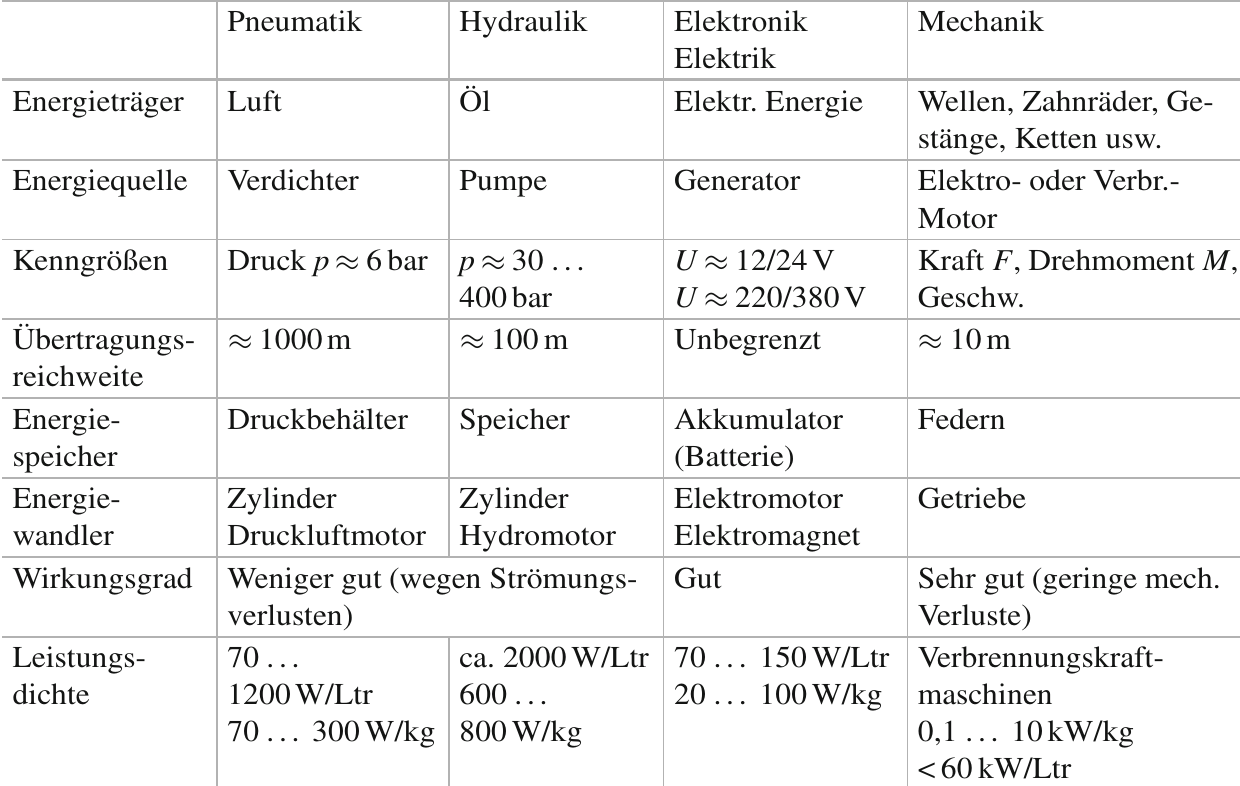
\includegraphics[width=\linewidth]{./ch01.basics/pics/compareDrives}  
  
  \vspace*{-1.0\baselineskip}{\tiny\color{red}Aus Sicherheitsgr\"unden wird bei der Pneumatik kein h\"oherer Druck 
  verwendet.}
  %%= = = = = = = = = = = = = = = = = = = = = = = = = = = = = = = = = = = = = =

\end{frame}
%= = = = = = = = = = = = = = = = = = = = = = = = = = = = = = = = = = = = = = =

% \part{Kombi}
% \section{Hydraulische und Pneumatische Bauteile}
\subsection{Grundlagen}
%= = = = = = = = = = = = = = = = = = = = = = = = = = = = = = = = = = = = = = =
%= = = = = = = = = = = = = = = = = = = = = = = = = = = = = = = = = = = = = = =
% \iffalse
\begin{frame}
  \frametitle{Eigenschaften der Fluide}
%  \framesubtitle{H\"oren}
  %%= = = = = = = = = = = = = = = = = = = = = = = = = = = = = = = = = = = = = =
  Anforderungen
  \begin{itemize}
    \item Temperatur-\adSTField{Viskosit\"ats}verhalten,
    \item gute Schmier- und \adSTField{Verschlei\ss{}schutz}eigenschaften 
      (h\"aufig Mischreibungsbedingungen bei kleinen Gleitgeschwindigkeiten),
    \item gute \adSTField{Korrosionsschutz}eigenschaften und gute 
      Lack- und Dichtungsvertr\"aglichkeit (Gummi, Kunststoffe, Buntmetalle),
    \item Alterungsbest\"andigkeit (\adSTField{Oxidation}, Harzbildung durch Polymerisation)
  \end{itemize}
  
   \ifteacher%%
   \else%%
    %  \vspace*{-0.7\baselineskip}\hspace{\stretch{1}}\rotatebox[origin=lB]{180}{%%
     \vspace*{-1.0\baselineskip}\hspace{\stretch{1}}\rotatebox[origin=lB]{180}{%%
     \resizebox{0.9\linewidth}{!}{\parbox[t]{3.95\linewidth}{%%
    %  \tiny
   %   \vspace*{-0.7\baselineskip}\hspace*{0.95\linewidth-1cm}\makebox[0pt][l]{\rotatebox[origin=c]{180}{\resizebox{1cm}{!}{%
     Viskosit\"ats, Verschlei\ss{}schutz, Korrosionsschutz, Oxidation
     }}}
   \fi%%
  
  %%= = = = = = = = = = = = = = = = = = = = = = = = = = = = = = = = = = = = = =

\end{frame}
%= = = = = = = = = = = = = = = = = = = = = = = = = = = = = = = = = = = = = = =

% \part{Kombi}
% \section{Hydraulische und Pneumatische Bauteile}
% \subsection{Grundlagen}
%= = = = = = = = = = = = = = = = = = = = = = = = = = = = = = = = = = = = = = =
%= = = = = = = = = = = = = = = = = = = = = = = = = = = = = = = = = = = = = = =
% \iffalse
\begin{frame}
  \frametitle{Eigenschaften der Fluide: Dichte $\rho$}
%  \framesubtitle{H\"oren}
  %%= = = = = = = = = = = = = = = = = = = = = = = = = = = = = = = = = = = = = =
  \vspace{-2\baselineskip}
  \[
    \rho = \frac{m}{V}\quad \left[\unit{\frac{kg}{m^3}}\right]
  \]  
  Im technischen Gebrauch liegt die Dichte $\rho$ der verwendeten Fluiden 
  (Hydraulik\"ol oder Druckfl\"ussigkeit) bei 
  % \teacherfalse
  \adSTFieldm{\unitfrac[900]{kg}{m^3}}.

  Bei steigender Temperatur wird das Volumen bei gleichbleibender Masse 
  gr\"o\ss{}er, die Dichte verringert sich daher mit dem Volums\"anderungskoeffizient
  $\alpha$:
  \[-\frac{\Delta\rho}{\rho}\approx\frac{\Delta V}{V}=\alpha \cdot \Delta \theta;
  \quad \begin{array}[c]{@{}l@{}}
        \rho_\theta =\rho_{15^\circ{}\mathrm{C}}+\adSTFieldm{\Delta \rho} \approx 
        \rho_{15^\circ{}\mathrm{C}} \cdot (1-\adSTFieldm{\alpha\cdot\Delta \theta}) \\
        V_\theta =V_{15^\circ{}\mathrm{C}}+\adSTFieldm{\Delta V} = 
        V_{15^\circ{}\mathrm{C}} \cdot (1+\adSTFieldm{\alpha\cdot\Delta \theta}) \\
        \end{array}\]

  % \adRule{6}{9}      
  \parbox[t]{0.45\linewidth}{%
  \begin{tabular}[t]{@{}rl@{}}
    $V$ & \adSTField{Volumen}\\
    $\Delta V$ & Volums\adSTField{\"anderung}\\
    $\rho_{15^\circ{}\mathrm{C}}$ & \adSTField{Dichte} bei $\unit[15]{^\circ{}C}$\\
    $\rho_\theta$ & Dichte bei \adSTField{Temperatur} $\theta$
  \end{tabular}
  }\hspace{\stretch{1}}\parbox[t]{0.53\linewidth}{%
  F\"ur die meisten Hydraulik\"ole ist der Volumenkorrekturfaktor 
  $\alpha \approx \unitfrac[0.70\cdot10^{-3}]{1}{K}$
  }

   \ifteacher%%
   \else%%
    %  \vspace*{-0.7\baselineskip}\hspace{\stretch{1}}\rotatebox[origin=lB]{180}{%%
     \vspace*{-1.0\baselineskip}\hspace{\stretch{1}}\rotatebox[origin=lB]{180}{%%
     \resizebox{0.9\linewidth}{!}{\parbox[t]{3.95\linewidth}{%%
    %  \tiny
   %   \vspace*{-0.7\baselineskip}\hspace*{0.95\linewidth-1cm}\makebox[0pt][l]{\rotatebox[origin=c]{180}{\resizebox{1cm}{!}{%
     $\Delta \rho$, $\alpha\cdot\Delta \theta$, $\Delta V$, $\alpha\cdot\Delta \theta$
     $\unitfrac[900]{kg}{m^3}$, Volumen, \"anderung, Dichte, Temperatur, 
     }}}
   \fi%%
  
  %%= = = = = = = = = = = = = = = = = = = = = = = = = = = = = = = = = = = = = =

\end{frame}
%= = = = = = = = = = = = = = = = = = = = = = = = = = = = = = = = = = = = = = =

% \part{Kombi}
% \section{Hydraulische und Pneumatische Bauteile}
% \subsection{Grundlagen}
%= = = = = = = = = = = = = = = = = = = = = = = = = = = = = = = = = = = = = = =
%= = = = = = = = = = = = = = = = = = = = = = = = = = = = = = = = = = = = = = =
% \iffalse
\begin{frame}
  \frametitle{Eigenschaften der Fluide: Dichte $\rho$}
%  \framesubtitle{H\"oren}
  %%= = = = = = = = = = = = = = = = = = = = = = = = = = = = = = = = = = = = = =
  \begin{block}{Beispiel: Dichte\"anderung bei Temperaturerh\"ohung}
    Bsp.: $\unit[2.5]{kg}$ eines Hydraulik\"oles mit einer Dichte von 
    $\unitfrac[900]{kg}{m^3}$ bei $\unit[15]{^\circ\,C}$ wird auf 
    $\unit[95]{^\circ\,C}$ erwärmt.
  Bestimmen Sie das Volumen.

  \end{block}


   \ifteacher%%
   \else%%
    %  \vspace*{-0.7\baselineskip}\hspace{\stretch{1}}\rotatebox[origin=lB]{180}{%%
     \vspace*{-1.0\baselineskip}\hspace{\stretch{1}}\rotatebox[origin=lB]{180}{%%
     \resizebox{0.9\linewidth}{!}{\parbox[t]{3.95\linewidth}{%%
    %  \tiny
   %   \vspace*{-0.7\baselineskip}\hspace*{0.95\linewidth-1cm}\makebox[0pt][l]{\rotatebox[origin=c]{180}{\resizebox{1cm}{!}{%
     \ %%
     }}}
   \fi%%
  
  %%= = = = = = = = = = = = = = = = = = = = = = = = = = = = = = = = = = = = = =

\end{frame}
%= = = = = = = = = = = = = = = = = = = = = = = = = = = = = = = = = = = = = = =

% \part{Kombi}
% \section{Hydraulische und Pneumatische Bauteile}
% \subsection{Grundlagen}
%= = = = = = = = = = = = = = = = = = = = = = = = = = = = = = = = = = = = = = =
%= = = = = = = = = = = = = = = = = = = = = = = = = = = = = = = = = = = = = = =
% \iffalse
\begin{frame}
  \frametitle{Eigenschaften der Fluide: Kompressibilit\"at}
%  \framesubtitle{H\"oren}
  %%= = = = = = = = = = = = = = = = = = = = = = = = = = = = = = = = = = = = = =
  Bei zunehmendem Druck komprimiert sich das \"Ol, der Zusammenhang 
  f\"ur das Dichte-Druck-Verhalten ist im linearisiertem Modell:

  \[
    \frac{\Delta\rho}{\rho}\approx-\frac{\Delta V}{V}=\beta \cdot \Delta p;
    \quad \begin{array}[c]{@{}l@{}}
      \rho_p =\rho_{p_0}+\adSTFieldm{\Delta \rho} \approx 
      \rho_{p_0} \cdot (1+\adSTFieldm{\beta\cdot\Delta p})     \\
      V_p =V_{p_0}+\adSTFieldm{\Delta V} = 
      V_{p_0} \cdot (1-\adSTFieldm{\beta\cdot\Delta p}) \\
      \end{array}
  \]


  \begin{tabular}[t]{@{}rl@{}}
    $V$ & \adSTField{Volumen}\\
    $\Delta V$ & Volums\adSTField{\"anderung}\\
    $\rho_{p_0}$ & \adSTField{Dichte} bei Normaldruck $p_0$\\
    $\rho_p$ & Dichte bei veränderten \adSTField{Druck} $p$\\
    $\beta$ &  \adSTField{Kompressibilit\"at}/Pressziffer in $\left[\unitfrac[]{1}{bar}\right]$\\
    $K=\nicefrac[]{1}{\beta}$ & Kompressionsmodul/\adSTField{Elastizit\"atsmodul} in $\left[\unit[]{bar}\right]$ 
  \end{tabular}

   \ifteacher%%
   \else%%
    %  \vspace*{-0.7\baselineskip}\hspace{\stretch{1}}\rotatebox[origin=lB]{180}{%%
     \vspace*{-1.0\baselineskip}\hspace{\stretch{1}}\rotatebox[origin=lB]{180}{%%
     \resizebox{0.9\linewidth}{!}{\parbox[t]{3.95\linewidth}{%%
    %  \tiny
   %   \vspace*{-0.7\baselineskip}\hspace*{0.95\linewidth-1cm}\makebox[0pt][l]{\rotatebox[origin=c]{180}{\resizebox{1cm}{!}{%
     $\Delta \rho$, $\beta\cdot\Delta p$, $\Delta V$, $\beta\cdot\Delta p$,\\
     Volumen, \"anderung, Dichte, Druck, Kompressibilit\"at, Elastizit\"atsmodul
     }}}
   \fi%%
  
  %%= = = = = = = = = = = = = = = = = = = = = = = = = = = = = = = = = = = = = =

\end{frame}
%= = = = = = = = = = = = = = = = = = = = = = = = = = = = = = = = = = = = = = =

% \part{Kombi}
% \section{Hydraulische und Pneumatische Bauteile}
% \subsection{Grundlagen}
%= = = = = = = = = = = = = = = = = = = = = = = = = = = = = = = = = = = = = = =
%= = = = = = = = = = = = = = = = = = = = = = = = = = = = = = = = = = = = = = =
% \iffalse
\begin{frame}
  \frametitle{Eigenschaften der Fluide: Kompressibilit\"at}
%  \framesubtitle{H\"oren}
  %%= = = = = = = = = = = = = = = = = = = = = = = = = = = = = = = = = = = = = =

  \begin{block}{Beispiel: Dichte\"anderung unter Druck}
    Bsp.: $\unit[2.5]{kg}$ eines Hydraulik\"oles mit einer Dichte von 
    $\unitfrac[900]{kg}{m^3}$ bei einem Druck von $p_0=\unit[1]{bar}$ 
    wird unter einen Druck von $p=\unit[150]{bar}$ komprimiert.
  Bestimmen Sie das Volumen.

  \begin{tabular}[]{@{}rll}
    \toprule
    & Kompressionsmodul $K$ & Kompressibilität $\beta$\\
    \"Olsorte & in $10^4$ bar & in $10^{-4}$ \unitfrac[]{1}{bar} \\
    \midrule
    Mineral\"ol &1.4 & 0.7\\
    HFC, HFD-Hydraulik\"ol & 3 & \nicefrac{1}{3} $\approx$ 0.33\\
    \bottomrule
  \end{tabular}

  Aus \emph{Hydraulik und Pneumatik, 2017}
  \end{block}


   \ifteacher%%
   \else%%
    %  \vspace*{-0.7\baselineskip}\hspace{\stretch{1}}\rotatebox[origin=lB]{180}{%%
     \vspace*{-1.0\baselineskip}\hspace{\stretch{1}}\rotatebox[origin=lB]{180}{%%
     \resizebox{0.9\linewidth}{!}{\parbox[t]{3.95\linewidth}{%%
    %  \tiny
   %   \vspace*{-0.7\baselineskip}\hspace*{0.95\linewidth-1cm}\makebox[0pt][l]{\rotatebox[origin=c]{180}{\resizebox{1cm}{!}{%
     Volumen, \"anderung, Dichte, Temperatur, $\unitfrac[900]{kg}{m^3}$
     }}}
   \fi%%
  
  %%= = = = = = = = = = = = = = = = = = = = = = = = = = = = = = = = = = = = = =

\end{frame}
%= = = = = = = = = = = = = = = = = = = = = = = = = = = = = = = = = = = = = = =

% \part{Kombi}
% \section{Hydraulische und Pneumatische Bauteile}
% \subsection{Grundlagen}
%= = = = = = = = = = = = = = = = = = = = = = = = = = = = = = = = = = = = = = =
%= = = = = = = = = = = = = = = = = = = = = = = = = = = = = = = = = = = = = = =
% \iffalse
\begin{frame}
  \frametitle{Eigenschaften der Fluide: Viskosit\"at, \emph{Rheologie}}
%  \framesubtitle{H\"oren}
  %%= = = = = = = = = = = = = = = = = = = = = = = = = = = = = = = = = = = = = =
  
  Die Viskosit\"at ist ein Ma\ss{} f\"ur den \adSTField{Flie\ss{}widerstand}, die Z\"ahigkeit
  auf Grund der inneren \adSTField{Reibung} (dick- und d\"unnfl\"ussg).

  \parbox[c]{0.49\linewidth}{
    In einem linearem \adSTField{Modell} (nach \textsc{Isaac NEWTON} werden zwei parallele 
    Platten mit einer \adSTField{Fl\"ache} $A$,
    die sich mit einer \adSTField{Relativgeschwindigkeit} $v$ zueinander bewegen und 
    in einem \adSTField{Abstand} $d=\Delta y$ sind, betrachtet.
  }\hspace{\stretch{1}}\parbox[c]{0.49\linewidth}{
      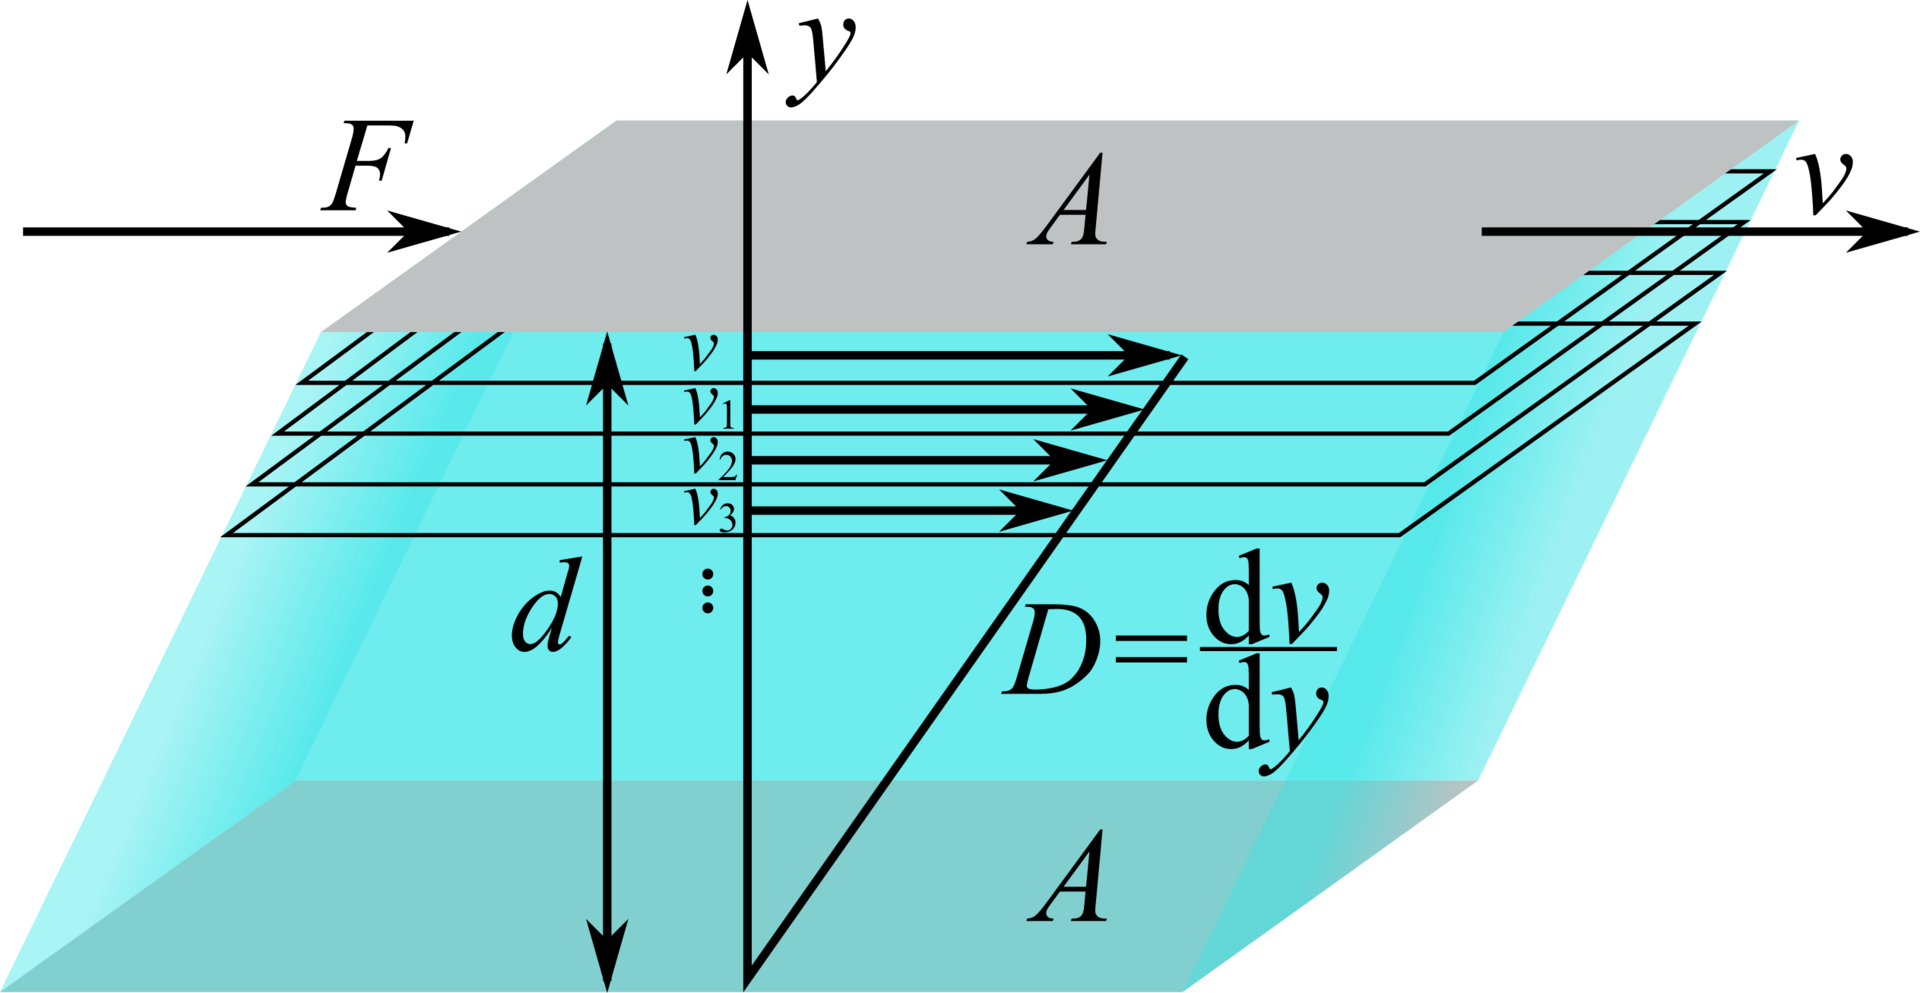
\includegraphics[width=\linewidth]{./ch01.basics/pics/Definition_Viskositaet}
  } 

  \ifteacher%%
  \else%%
   %  \vspace*{-0.7\baselineskip}\hspace{\stretch{1}}\rotatebox[origin=lB]{180}{%%
    \vspace*{-0.0\baselineskip}\hspace{\stretch{1}}\rotatebox[origin=lB]{180}{%%
    \resizebox{0.9\linewidth}{!}{\parbox[t]{3.95\linewidth}{%%
   %  \tiny
  %   \vspace*{-0.7\baselineskip}\hspace*{0.95\linewidth-1cm}\makebox[0pt][l]{\rotatebox[origin=c]{180}{\resizebox{1cm}{!}{%
  Flie\ss{}widerstand, Reibung, Modell, Fl\"ache, Relativgeschwindigkeit, Abstand
    }}}
  \fi%%
  
  %%= = = = = = = = = = = = = = = = = = = = = = = = = = = = = = = = = = = = = =

\end{frame}
%= = = = = = = = = = = = = = = = = = = = = = = = = = = = = = = = = = = = = = =

% \part{Kombi}
% \section{Hydraulische und Pneumatische Bauteile}
% \subsection{Grundlagen}
%= = = = = = = = = = = = = = = = = = = = = = = = = = = = = = = = = = = = = = =
%= = = = = = = = = = = = = = = = = = = = = = = = = = = = = = = = = = = = = = =
% \iffalse
\begin{frame}
  \frametitle{Eigenschaften der Fluide: Viskosit\"at, \emph{Rheologie}}
%  \framesubtitle{H\"oren}
  %%= = = = = = = = = = = = = = = = = = = = = = = = = = = = = = = = = = = = = =
  
  \begin{tabular}[t]{@{}lll@{}}
    je gr\"o\ss{}er die Fl\"ache & desto \adSTField{gr\"o\ss{}er} die Kraft & $F\sim A$\\
    je gr\"o\ss{}er die Geschwindigkeit & desto \adSTField{gr\"o\ss{}er} die Kraft & $F\sim \Delta v\ (\diff{v})$\\
    je gr\"o\ss{}er der Abstand der Platten & desto \adSTField{kleiner} die Kraft & $F \sim \nicefrac[]{1}{\Delta y}\ (\nicefrac[]{1}{\diff{y}})$
  \end{tabular}
  

  Mit dem materialabh\"angigen Proportionalit\"atfaktor $\eta$ 
  (absolute oder dynamische Viskosit\"at) erh\"alt man (im einfachen linearen Modell):
  \parbox[c]{0.49\linewidth}{
    \[
      F = \eta \cdot A \cdot \frac{\Delta v}{\Delta y}= \eta \cdot A \cdot \frac{\diff{v}}{\diff{y}}
    \] 
  }\hspace{\stretch{1}}\parbox[c]{0.49\linewidth}{
    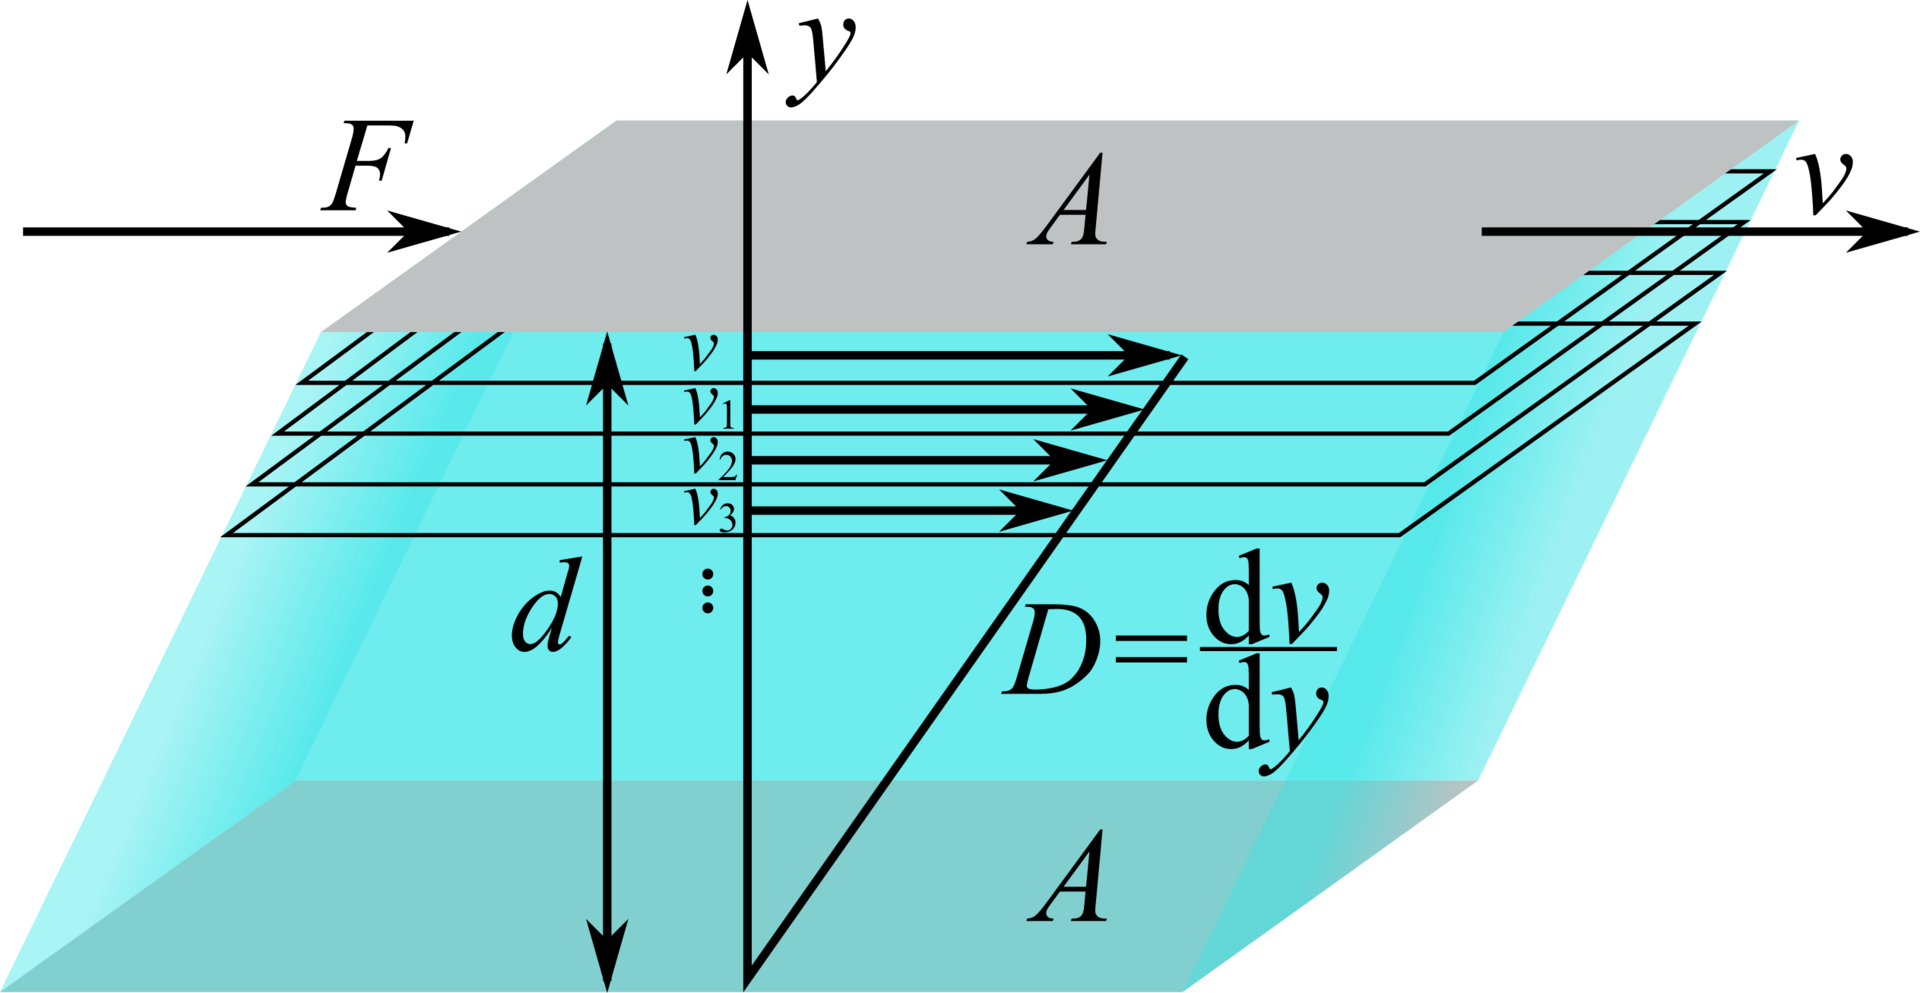
\includegraphics[width=\linewidth]{./ch01.basics/pics/Definition_Viskositaet}
  }

  \ifteacher%%
  \else%%
   %  \vspace*{-0.7\baselineskip}\hspace{\stretch{1}}\rotatebox[origin=lB]{180}{%%
    \vspace*{-1.0\baselineskip}\hspace{\stretch{1}}\rotatebox[origin=lB]{180}{%%
    \resizebox{0.9\linewidth}{!}{\parbox[t]{3.95\linewidth}{%%
   %  \tiny
  %   \vspace*{-0.7\baselineskip}\hspace*{0.95\linewidth-1cm}\makebox[0pt][l]{\rotatebox[origin=c]{180}{\resizebox{1cm}{!}{%
  gr\"o\ss{}er, gr\"o\ss{}er, kleiner
    }}}
  \fi%%

  % \begin{block}{Beispiel: Dichte\"anderung unter Druck}
  %   Bsp.: $\unit[2.5]{kg}$ eines Hydraulik\"oles mit einer Dichte von 
  %   $\unitfrac[900]{kg}{m^3}$ bei einem Druck von $p_0=\unit[1]{bar}$ 
  %   wird unter einen Druck von $p=\unit[150]{bar}$ komprimiert.
  % Bestimmen Sie das Volumen.

  %%= = = = = = = = = = = = = = = = = = = = = = = = = = = = = = = = = = = = = =

\end{frame}
%= = = = = = = = = = = = = = = = = = = = = = = = = = = = = = = = = = = = = = =

% \part{Kombi}
% \section{Hydraulische und Pneumatische Bauteile}
% \subsection{Grundlagen}
%= = = = = = = = = = = = = = = = = = = = = = = = = = = = = = = = = = = = = = =
%= = = = = = = = = = = = = = = = = = = = = = = = = = = = = = = = = = = = = = =
% \iffalse
\begin{frame}
  \frametitle{Eigenschaften der Fluide: Viskosit\"at, \emph{Rheologie}}
%  \framesubtitle{H\"oren}
  %%= = = = = = = = = = = = = = = = = = = = = = = = = = = = = = = = = = = = = =
  Die Viskosit\"at \"andert sich mit:
  \begin{itemize}
    \item \adSTField{Temperatur}
    \item \adSTField{Druck}
    \item \adSTField{Geschwindigkeit}
    \item Alterung
  \end{itemize}
  
  Durch Zugabe von Additiven wird versucht, die Eigenschaften des Hydraulik\"oles
  f\"ur den Betrieb zu verbessern, und Alterungsvorg\"ange zu verlangsamen.

  \ifteacher%%
  \else%%
   %  \vspace*{-0.7\baselineskip}\hspace{\stretch{1}}\rotatebox[origin=lB]{180}{%%
    \vspace*{-1.0\baselineskip}\hspace{\stretch{1}}\rotatebox[origin=lB]{180}{%%
    \resizebox{0.9\linewidth}{!}{\parbox[t]{3.95\linewidth}{%%
   %  \tiny
  %   \vspace*{-0.7\baselineskip}\hspace*{0.95\linewidth-1cm}\makebox[0pt][l]{\rotatebox[origin=c]{180}{\resizebox{1cm}{!}{%
  Temperatur, Druck, Geschwindigkeit
    }}}
  \fi%%

  % \begin{block}{Beispiel: Dichte\"anderung unter Druck}
  %   Bsp.: $\unit[2.5]{kg}$ eines Hydraulik\"oles mit einer Dichte von 
  %   $\unitfrac[900]{kg}{m^3}$ bei einem Druck von $p_0=\unit[1]{bar}$ 
  %   wird unter einen Druck von $p=\unit[150]{bar}$ komprimiert.
  % Bestimmen Sie das Volumen.

  %%= = = = = = = = = = = = = = = = = = = = = = = = = = = = = = = = = = = = = =

\end{frame}
%= = = = = = = = = = = = = = = = = = = = = = = = = = = = = = = = = = = = = = =



% \part{Kombi}
% \section{Hydraulische und Pneumatische Bauteile}
% \subsection{Grundlagen}
%= = = = = = = = = = = = = = = = = = = = = = = = = = = = = = = = = = = = = = =
%= = = = = = = = = = = = = = = = = = = = = = = = = = = = = = = = = = = = = = =
% \iffalse
\begin{frame}
  \frametitle{Kennbuchstaben }
%  \framesubtitle{H\"oren}
  %%= = = = = = = = = = = = = = = = = = = = = = = = = = = = = = = = = = = = = =
  \begin{tabular}[t]{@{}ll@{\quad}ll@{}}
    \toprule
    AN  & Normalschmieröle,                    & Jx  & elektrische Isolieröle,             \\
    Bx  & Schmieröl BA, BB oder                &     & JA oder JB,                         \\
        & BC (z. B.: bitumenhaltig),           & Kx  & Kältemaschinenöle,                  \\
    C   & Umlaufschmieröle,                    & L   & Härte- und Vergüteöle,              \\
    CG  & Gleitbahnöle,                        & Q   & Wärmeträgeröle,                     \\
    D   & Druckluftöle,                        & R   & Korrosionsschutzöle,                \\
    F   & Luftfilteröle,                       & S   & Kühlschmierstoffe,                  \\
    FS  & Formen-Trennöle,                     & TD  & Schmier- und Regleröle,             \\
    H   & Hydrauliköle,                        & V   & Luftverdichteröle,                  \\
    HF  & schwer entflammbare Hydraulik\"ole,  & W   & Walzöle,                            \\
    HE  & biologisch abbaubare Hydraulik\"ole, & Zx  & Dampfzylinderöle.                   \\ 
    HV  & Hydrauliköle mit verbessertem        &     & ZS, ZA, ZB oder ZD.\\
        & Viskositäts-Temperatur-Verhalten, \\
    \bottomrule
  \end{tabular}

  \ifteacher%%
  \else%%
   %  \vspace*{-0.7\baselineskip}\hspace{\stretch{1}}\rotatebox[origin=lB]{180}{%%
    \vspace*{-1.0\baselineskip}\hspace{\stretch{1}}\rotatebox[origin=lB]{180}{%%
    \resizebox{0.9\linewidth}{!}{\parbox[t]{3.95\linewidth}{%%
   %  \tiny
  %   \vspace*{-0.7\baselineskip}\hspace*{0.95\linewidth-1cm}\makebox[0pt][l]{\rotatebox[origin=c]{180}{\resizebox{1cm}{!}{%
  Temperatur, Druck, Geschwindigkeit
    }}}
  \fi%%

  % \begin{block}{Beispiel: Dichte\"anderung unter Druck}
  %   Bsp.: $\unit[2.5]{kg}$ eines Hydraulik\"oles mit einer Dichte von 
  %   $\unitfrac[900]{kg}{m^3}$ bei einem Druck von $p_0=\unit[1]{bar}$ 
  %   wird unter einen Druck von $p=\unit[150]{bar}$ komprimiert.
  % Bestimmen Sie das Volumen.

  %%= = = = = = = = = = = = = = = = = = = = = = = = = = = = = = = = = = = = = =

\end{frame}
%= = = = = = = = = = = = = = = = = = = = = = = = = = = = = = = = = = = = = = =



% \part{Kombi}
% \section{Intro}
% \subsection*{Intro}
% %= = = = = = = = = = = = = = = = = = = = = = = = = = = = = = = = = = = = = = =
% %= = = = = = = = = = = = = = = = = = = = = = = = = = = = = = = = = = = = = = =
% % \iffalse
% \begin{frame}
%   \frametitle{Intro}
% %  \framesubtitle{H\"oren}
%   %%= = = = = = = = = = = = = = = = = = = = = = = = = = = = = = = = = = = = = =
%   Todo
%   what ist
%   %%= = = = = = = = = = = = = = = = = = = = = = = = = = = = = = = = = = = = = =
%
% \end{frame}
% %= = = = = = = = = = = = = = = = = = = = = = = = = = = = = = = = = = = = = = =

% \part{Kombi}
\section{Intro}
% \subsection*{Intro}
% \input{ch04.matrices/chapter/matrices.intro.tex}
